\documentclass[tikz]{standalone}
\usepackage{amsmath}
\usepackage{tikz}

\begin{document}

\begin{figure}[h]
\begin{center}
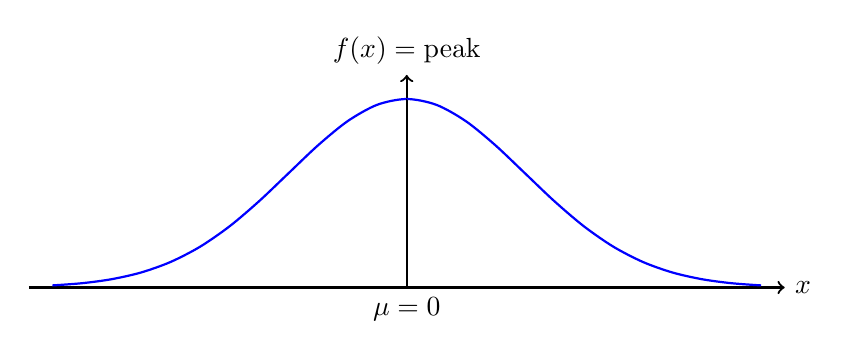
\begin{tikzpicture}[xscale=1.5, yscale=6]
  \draw[->, thick] (-3.2,0) -- (3.2,0) node[right] {$x$};
  \draw[->, thick] (0,0) -- (0,0.45) node[above] {$f(x) = \text{peak}$};

  \draw[domain=-3:3, smooth, variable=\x, blue, thick] 
    plot ({\x}, {1/sqrt(2*pi) * exp(-0.5*\x*\x)});

  \draw[dashed] (0,0) -- (0,{1/sqrt(2*pi)});
  \node[below] at (0,0) {$\mu = 0$};
\end{tikzpicture}
\end{center}
\caption{An illustration of symmetric distribution. Area under this curve on the left hand side of $\mu = 0$ is same as the area on the right hand side under the curve.}
\end{figure}
\end{document}